\subsection{End-to-End Latency Analysis}

The end-to-end processing pipeline was analyzed to quantify the latency introduced by each architectural layer, from the user's intent submission at the Frontend to the enforcement at the E2 Node. Figure \ref{fig:proc_time} illustrates the mean processing times for each stage. The total latency is dominated by the Service Management and Orchestration (SMO) layer, specifically the stochastic processing within the Large Language Model (LLM) components. The translation of natural language intents into policy artifacts (\textit{SMO Intent$\to$Policy}) and the subsequent tool execution (\textit{SMO MCP Tool Execution}) exhibit significant duration compared to the downstream components, contributing the majority of the total end-to-end delay.

In contrast to the SMO layer, the Near-RT RIC and E2 Node components demonstrate highly deterministic behavior with minimal variance. The xApp processing time (\textit{xApp Full Policy Processing}) and the A1 Mediator latency remain consistently low, validating the platform's suitability for near-real-time control loops. The variance observed in the upper layers, indicated by the error bars in Figure \ref{fig:proc_time}, is inherent to the generative nature of the LLM and network conditions during the initial REST interactions. Conversely, the strict timing requirements of the O-RAN specification are met by the lower layers, where the control loop operations (\textit{xApp Policy$\to$Control} and \textit{E2 Node Control Processing}) execute within the sub-second/millisecond range required for effective RAN optimization.

\begin{figure}[htbp]
    \centering
    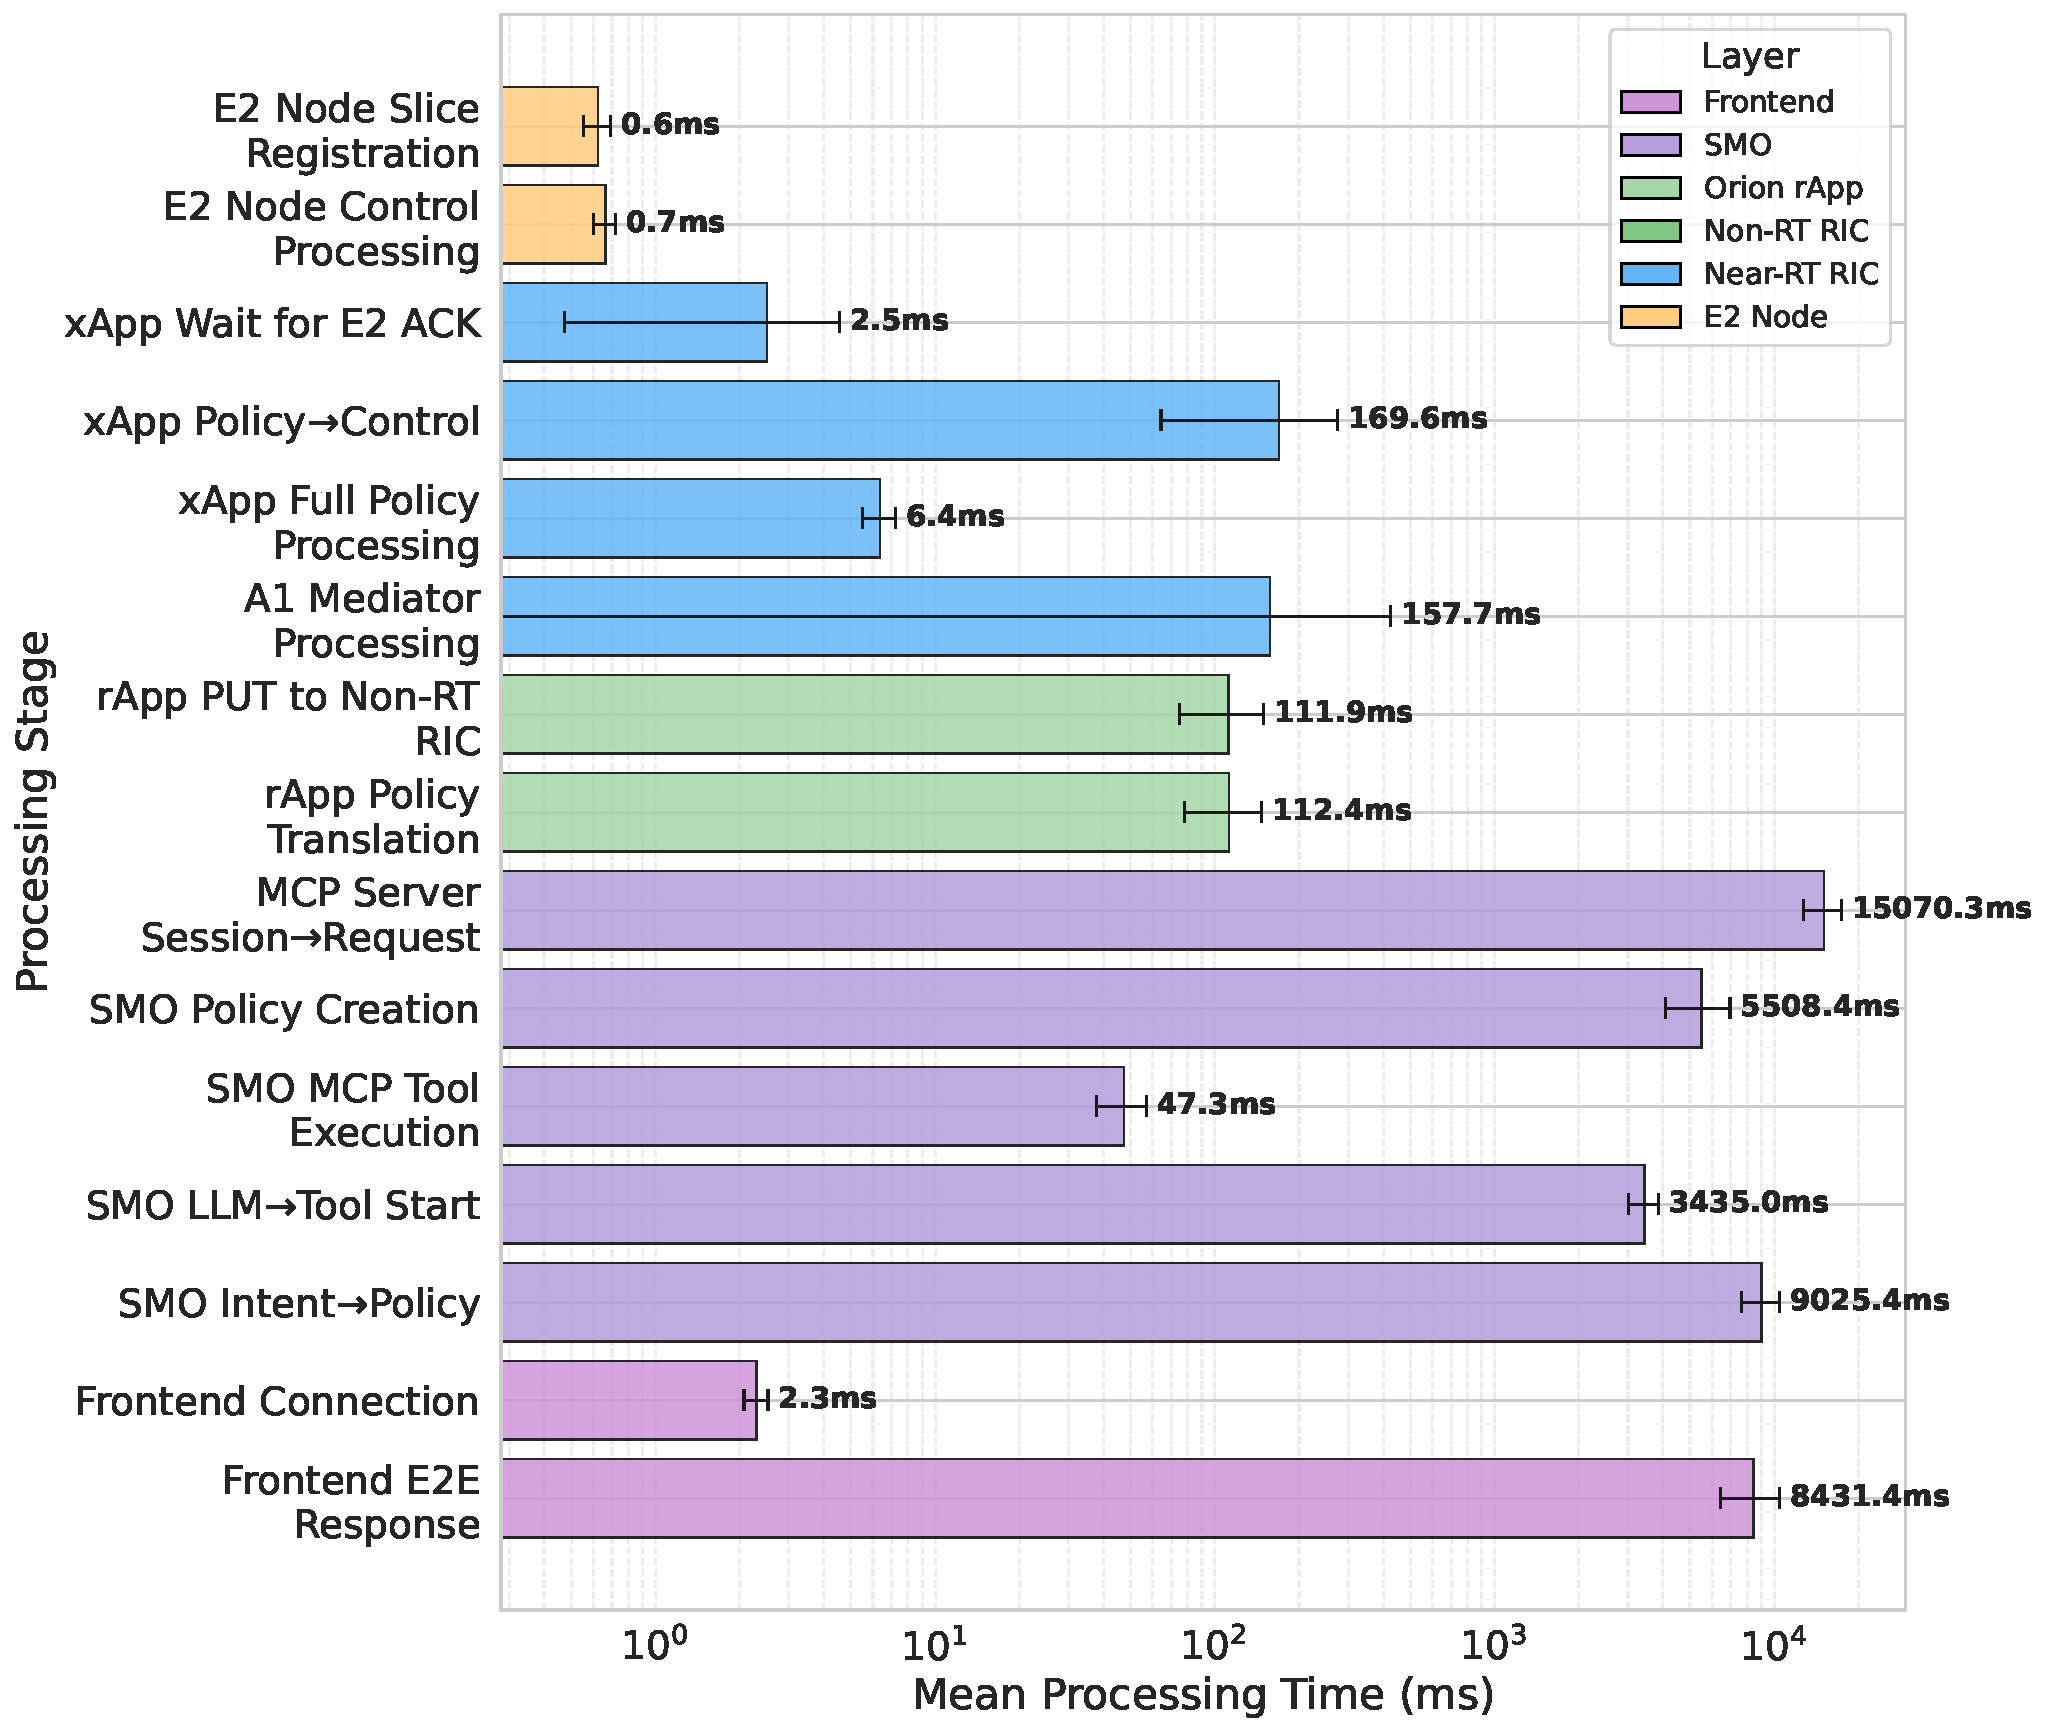
\includegraphics[width=\linewidth]{times/processing_time_by_stage.pdf}
    \caption{Mean processing time breakdown across O-RAN architectural layers. The diagram highlights the latency disparity between the compute-intensive intent processing in the SMO (purple) and the highly optimized, deterministic control operations in the Near-RT RIC (blue) and E2 Node (orange). Error bars indicate standard deviation.}
    \label{fig:proc_time}
\end{figure}
